% ============================================================================
% SEC02.TEX - Section 2.2: Instalasi dan Setup
% ============================================================================

\section{Instalasi dan Setup Unity}

\begin{learningoutcomes}
\item Mampu mengunduh dan menginstal Unity Hub
\item Mampu menginstal Unity Editor
\item Memahami konfigurasi project Unity
\item Mampu membuat project Unity pertama
\end{learningoutcomes}

\subsection{Unity Hub}

Unity Hub adalah aplikasi manajemen untuk Unity yang memungkinkan:
\begin{itemize}
\item Menginstal berbagai versi Unity
\item Mengelola project Unity
\item Mengakses Unity Learn dan resources
\end{itemize}

\begin{figure}[ht]
    \centering
    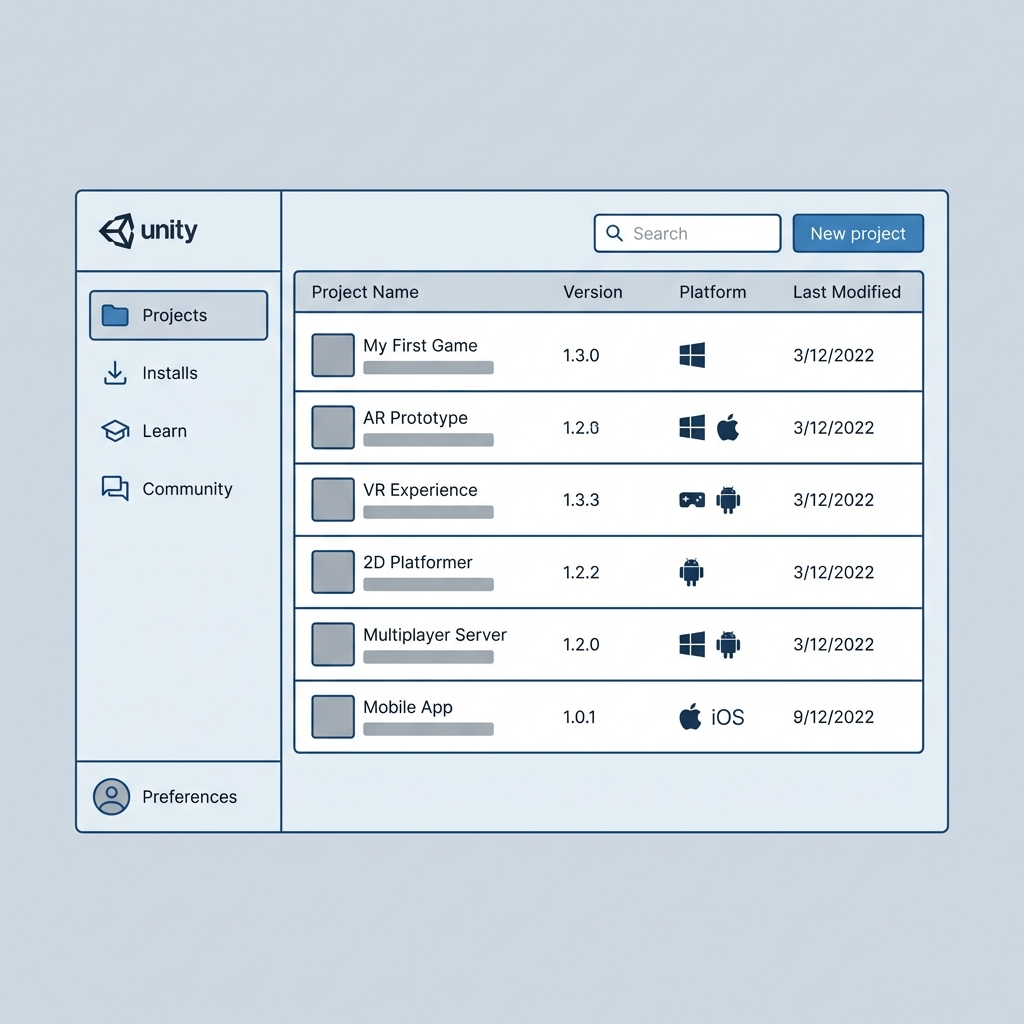
\includegraphics[width=0.8\textwidth]{figures/unity_hub.png}
    \caption{Antarmuka Unity Hub}
    \label{fig:unity_hub}
\end{figure}

\subsection{Langkah Instalasi}

\begin{enumerate}
\item \textbf{Download Unity Hub}: Kunjungi unity.com/download
\item \textbf{Install Unity Hub}: Jalankan installer
\item \textbf{Login/Register}: Buat akun Unity (gratis)
\item \textbf{Install Unity Editor}: Pilih versi LTS (Long Term Support) yang stabil
\item \textbf{Install Modules}: Pilih platform target (Windows, Android, iOS, dll)
\end{enumerate}

\subsection{Membuat Project Baru}

\begin{enumerate}
\item Buka Unity Hub
\item Klik "New Project"
\item Pilih template (2D, 3D, atau lainnya)
\item Tentukan nama dan lokasi project
\item Klik "Create Project"
\end{enumerate}

\begin{catatan}
Untuk pembelajaran, gunakan template 3D atau 2D. Template lain seperti VR atau Mobile dapat dipilih sesuai kebutuhan spesifik.
\end{catatan}

\subsection{Struktur Folder Project}

Setelah project dibuat, Unity membuat struktur folder:
\begin{itemize}
\item \textbf{Assets/}: Semua assets game (scripts, models, textures, dll)
\item \textbf{Library/}: File cache Unity (jangan di-edit manual)
\item \textbf{Logs/}: Log files
\item \textbf{Packages/}: Package manifest
\item \textbf{ProjectSettings/}: Pengaturan project
\end{itemize}

\subsection{Konfigurasi Awal}

\textbf{Project Settings Penting}:
\begin{itemize}
\item \textbf{Player Settings}: Nama aplikasi, icon, splash screen
\item \textbf{Graphics Settings}: Rendering pipeline, quality settings
\item \textbf{Input Manager}: Input configuration
\item \textbf{Physics Settings}: Gravity, timestep, dll
\end{itemize}
